% Options for packages loaded elsewhere
\PassOptionsToPackage{unicode}{hyperref}
\PassOptionsToPackage{hyphens}{url}
%
\documentclass[
]{article}
\usepackage{lmodern}
\usepackage{amssymb,amsmath}
\usepackage{ifxetex,ifluatex}
\ifnum 0\ifxetex 1\fi\ifluatex 1\fi=0 % if pdftex
  \usepackage[T1]{fontenc}
  \usepackage[utf8]{inputenc}
  \usepackage{textcomp} % provide euro and other symbols
\else % if luatex or xetex
  \usepackage{unicode-math}
  \defaultfontfeatures{Scale=MatchLowercase}
  \defaultfontfeatures[\rmfamily]{Ligatures=TeX,Scale=1}
\fi
% Use upquote if available, for straight quotes in verbatim environments
\IfFileExists{upquote.sty}{\usepackage{upquote}}{}
\IfFileExists{microtype.sty}{% use microtype if available
  \usepackage[]{microtype}
  \UseMicrotypeSet[protrusion]{basicmath} % disable protrusion for tt fonts
}{}
\makeatletter
\@ifundefined{KOMAClassName}{% if non-KOMA class
  \IfFileExists{parskip.sty}{%
    \usepackage{parskip}
  }{% else
    \setlength{\parindent}{0pt}
    \setlength{\parskip}{6pt plus 2pt minus 1pt}}
}{% if KOMA class
  \KOMAoptions{parskip=half}}
\makeatother
\usepackage{xcolor}
\IfFileExists{xurl.sty}{\usepackage{xurl}}{} % add URL line breaks if available
\IfFileExists{bookmark.sty}{\usepackage{bookmark}}{\usepackage{hyperref}}
\hypersetup{
  pdftitle={LM Homework 2},
  pdfauthor={Joshua Ingram},
  hidelinks,
  pdfcreator={LaTeX via pandoc}}
\urlstyle{same} % disable monospaced font for URLs
\usepackage[margin=1in]{geometry}
\usepackage{color}
\usepackage{fancyvrb}
\newcommand{\VerbBar}{|}
\newcommand{\VERB}{\Verb[commandchars=\\\{\}]}
\DefineVerbatimEnvironment{Highlighting}{Verbatim}{commandchars=\\\{\}}
% Add ',fontsize=\small' for more characters per line
\usepackage{framed}
\definecolor{shadecolor}{RGB}{248,248,248}
\newenvironment{Shaded}{\begin{snugshade}}{\end{snugshade}}
\newcommand{\AlertTok}[1]{\textcolor[rgb]{0.94,0.16,0.16}{#1}}
\newcommand{\AnnotationTok}[1]{\textcolor[rgb]{0.56,0.35,0.01}{\textbf{\textit{#1}}}}
\newcommand{\AttributeTok}[1]{\textcolor[rgb]{0.77,0.63,0.00}{#1}}
\newcommand{\BaseNTok}[1]{\textcolor[rgb]{0.00,0.00,0.81}{#1}}
\newcommand{\BuiltInTok}[1]{#1}
\newcommand{\CharTok}[1]{\textcolor[rgb]{0.31,0.60,0.02}{#1}}
\newcommand{\CommentTok}[1]{\textcolor[rgb]{0.56,0.35,0.01}{\textit{#1}}}
\newcommand{\CommentVarTok}[1]{\textcolor[rgb]{0.56,0.35,0.01}{\textbf{\textit{#1}}}}
\newcommand{\ConstantTok}[1]{\textcolor[rgb]{0.00,0.00,0.00}{#1}}
\newcommand{\ControlFlowTok}[1]{\textcolor[rgb]{0.13,0.29,0.53}{\textbf{#1}}}
\newcommand{\DataTypeTok}[1]{\textcolor[rgb]{0.13,0.29,0.53}{#1}}
\newcommand{\DecValTok}[1]{\textcolor[rgb]{0.00,0.00,0.81}{#1}}
\newcommand{\DocumentationTok}[1]{\textcolor[rgb]{0.56,0.35,0.01}{\textbf{\textit{#1}}}}
\newcommand{\ErrorTok}[1]{\textcolor[rgb]{0.64,0.00,0.00}{\textbf{#1}}}
\newcommand{\ExtensionTok}[1]{#1}
\newcommand{\FloatTok}[1]{\textcolor[rgb]{0.00,0.00,0.81}{#1}}
\newcommand{\FunctionTok}[1]{\textcolor[rgb]{0.00,0.00,0.00}{#1}}
\newcommand{\ImportTok}[1]{#1}
\newcommand{\InformationTok}[1]{\textcolor[rgb]{0.56,0.35,0.01}{\textbf{\textit{#1}}}}
\newcommand{\KeywordTok}[1]{\textcolor[rgb]{0.13,0.29,0.53}{\textbf{#1}}}
\newcommand{\NormalTok}[1]{#1}
\newcommand{\OperatorTok}[1]{\textcolor[rgb]{0.81,0.36,0.00}{\textbf{#1}}}
\newcommand{\OtherTok}[1]{\textcolor[rgb]{0.56,0.35,0.01}{#1}}
\newcommand{\PreprocessorTok}[1]{\textcolor[rgb]{0.56,0.35,0.01}{\textit{#1}}}
\newcommand{\RegionMarkerTok}[1]{#1}
\newcommand{\SpecialCharTok}[1]{\textcolor[rgb]{0.00,0.00,0.00}{#1}}
\newcommand{\SpecialStringTok}[1]{\textcolor[rgb]{0.31,0.60,0.02}{#1}}
\newcommand{\StringTok}[1]{\textcolor[rgb]{0.31,0.60,0.02}{#1}}
\newcommand{\VariableTok}[1]{\textcolor[rgb]{0.00,0.00,0.00}{#1}}
\newcommand{\VerbatimStringTok}[1]{\textcolor[rgb]{0.31,0.60,0.02}{#1}}
\newcommand{\WarningTok}[1]{\textcolor[rgb]{0.56,0.35,0.01}{\textbf{\textit{#1}}}}
\usepackage{graphicx,grffile}
\makeatletter
\def\maxwidth{\ifdim\Gin@nat@width>\linewidth\linewidth\else\Gin@nat@width\fi}
\def\maxheight{\ifdim\Gin@nat@height>\textheight\textheight\else\Gin@nat@height\fi}
\makeatother
% Scale images if necessary, so that they will not overflow the page
% margins by default, and it is still possible to overwrite the defaults
% using explicit options in \includegraphics[width, height, ...]{}
\setkeys{Gin}{width=\maxwidth,height=\maxheight,keepaspectratio}
% Set default figure placement to htbp
\makeatletter
\def\fps@figure{htbp}
\makeatother
\setlength{\emergencystretch}{3em} % prevent overfull lines
\providecommand{\tightlist}{%
  \setlength{\itemsep}{0pt}\setlength{\parskip}{0pt}}
\setcounter{secnumdepth}{-\maxdimen} % remove section numbering

\title{LM Homework 2}
\author{Joshua Ingram}
\date{2/19/2020}

\begin{document}
\maketitle

\hypertarget{problem-1}{%
\section{Problem 1}\label{problem-1}}

\hypertarget{section}{%
\subsection{1.}\label{section}}

\begin{Shaded}
\begin{Highlighting}[]
\KeywordTok{head}\NormalTok{(Anscombe)}
\end{Highlighting}
\end{Shaded}

\begin{verbatim}
##    education income under18 urban
## ME       189   2824   350.7   508
## NH       169   3259   345.9   564
## VT       230   3072   348.5   322
## MA       168   3835   335.3   846
## RI       180   3549   327.1   871
## CT       193   4256   341.0   774
\end{verbatim}

\begin{Shaded}
\begin{Highlighting}[]
\KeywordTok{plot}\NormalTok{(Anscombe)}
\end{Highlighting}
\end{Shaded}

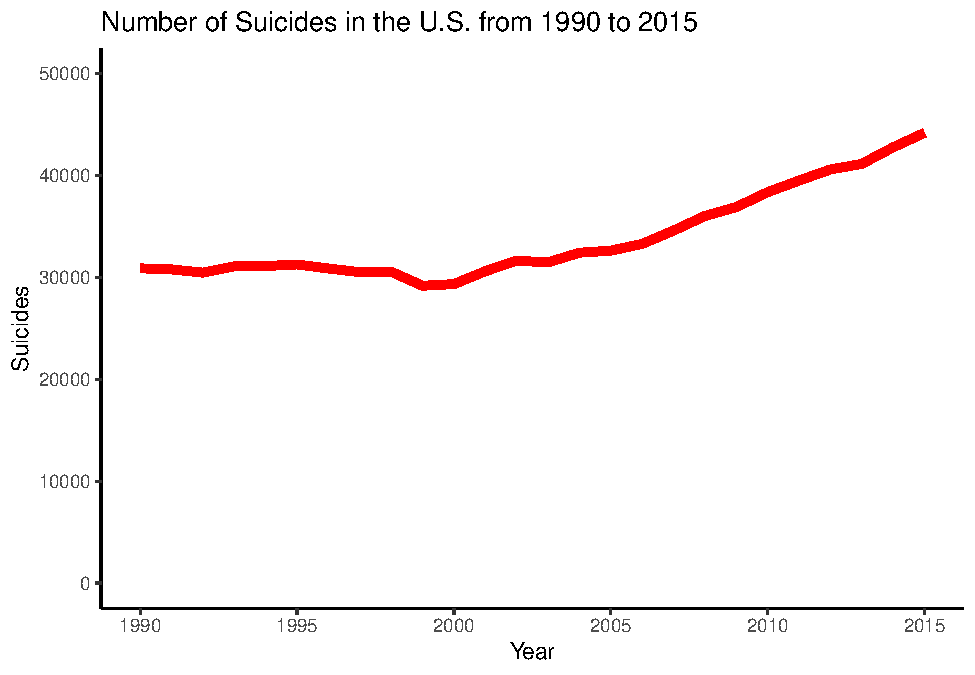
\includegraphics{LM-Homework-2_files/figure-latex/unnamed-chunk-1-1.pdf}

\begin{Shaded}
\begin{Highlighting}[]
\KeywordTok{cor}\NormalTok{(Anscombe)}
\end{Highlighting}
\end{Shaded}

\begin{verbatim}
##           education     income    under18      urban
## education 1.0000000  0.6675773  0.3114855  0.2633238
## income    0.6675773  1.0000000 -0.1623600  0.6854580
## under18   0.3114855 -0.1623600  1.0000000 -0.1386334
## urban     0.2633238  0.6854580 -0.1386334  1.0000000
\end{verbatim}

income seems to be the variable that has the strongest relationship with
education spendings.

\hypertarget{section-1}{%
\subsection{2.}\label{section-1}}

\begin{Shaded}
\begin{Highlighting}[]
\NormalTok{lm_edu1 <-}\StringTok{ }\KeywordTok{lm}\NormalTok{(education }\OperatorTok{~}\StringTok{ }\NormalTok{income, }\DataTypeTok{data =}\NormalTok{ Anscombe)}
\KeywordTok{summary}\NormalTok{(lm_edu1)}
\end{Highlighting}
\end{Shaded}

\begin{verbatim}
## 
## Call:
## lm(formula = education ~ income, data = Anscombe)
## 
## Residuals:
##     Min      1Q  Median      3Q     Max 
## -62.077 -21.868  -4.617  17.523 124.701 
## 
## Coefficients:
##              Estimate Std. Error t value Pr(>|t|)    
## (Intercept) 17.710031  28.873840   0.613    0.542    
## income       0.055376   0.008823   6.276 8.76e-08 ***
## ---
## Signif. codes:  0 '***' 0.001 '**' 0.01 '*' 0.05 '.' 0.1 ' ' 1
## 
## Residual standard error: 34.94 on 49 degrees of freedom
## Multiple R-squared:  0.4457, Adjusted R-squared:  0.4343 
## F-statistic: 39.39 on 1 and 49 DF,  p-value: 8.762e-08
\end{verbatim}

Equation: \(\hat{education_i} = 17.71 + 0.0554(income_i)\)

Interpretations:

slope: On average, we predict that there will be a \$0.055 increase in
per-capita education expenditures for every one dollar increase in
per-capita income.

intercept: When per-capita income is 0, we predict, on average, that the
per-capita education expenditures will be \$17.71. (not sure about the
full context of this data, but perhaps this is the per-capita income for
a given county, so if a county has close to 0 per-capita income, they
may still receive state/federal assistance? That's why I interpretted)

RSE: 34.94

interpretation: On average, our estimates for education expenditures
(per-capita) are off by 34.94 dollars

\(R^2:\) 0.4457

intperpretation: 44.57\% of the variance in education ependitures per
capita is explained by our model

\hypertarget{section-2}{%
\subsection{3.}\label{section-2}}

\hypertarget{a.}{%
\subsubsection{a.}\label{a.}}

\(\hat{education_i} = \hat{\beta_0} + \hat{\beta_1}(income_i) + \hat{\beta_2}(under18_i) + \hat{\beta_3}(urban_i) + \epsilon_i\)

\hypertarget{b.}{%
\subsubsection{b.}\label{b.}}

Find that:
\(\alpha = \bar{y} - \beta_1\bar{x_1} - \beta_2\bar{x_2} -\beta_3\bar{x_3}\)

\(\frac{\delta}{\delta\alpha} \Sigma( y_i - (\alpha + \beta_1x_1 + \beta_2x_2 + \beta_3x_3))^2\)

\(= \Sigma \frac{\delta}{\delta\alpha} ( y_i - (\alpha + \beta_1x_1 -+\beta_2x_2 +\beta_3x_3))^2\)

\(= \Sigma 2( y_i - (\alpha + - \beta_1x_1 - \beta_2x_2 -\beta_3x_3)(-1)\)

\(= \Sigma -2( y_i - (\alpha + \beta_1x_1 + \beta_2x_2 +\beta_3x_3) = 0\)

\(\Sigma ( y_i - (\alpha + \beta_1x_1 + \beta_2x_2 +\beta_3x_3) = 0\)

\(\Sigma y_i - \Sigma(\alpha + \beta_1x_1 + \beta_2x_2 +\beta_3x_3) = 0\)

\(\Sigma y_i - \Sigma\alpha - \Sigma\beta_1x_1 - \Sigma\beta_2x_2 - \Sigma\beta_3x_3) = 0\)

\(\Sigma y_i - n\alpha - \Sigma\beta_1x_1 - \Sigma\beta_2x_2 - \Sigma\beta_3x_3) = 0\)

\(\Sigma y_i - \Sigma\beta_1x_1 - \Sigma\beta_2x_2 - \Sigma\beta_3x_3) = n\alpha\)

\(\alpha = \bar{y} - \beta_1\bar{x_1} - \beta_2\bar{x_2} -\beta_3\bar{x_3}\)

\hypertarget{c.}{%
\subsubsection{c.}\label{c.}}

\begin{Shaded}
\begin{Highlighting}[]
\NormalTok{lm_edu2 <-}\StringTok{ }\KeywordTok{lm}\NormalTok{(education }\OperatorTok{~}\StringTok{ }\NormalTok{income }\OperatorTok{+}\StringTok{ }\NormalTok{under18 }\OperatorTok{+}\StringTok{ }\NormalTok{urban, }\DataTypeTok{data =}\NormalTok{ Anscombe)}
\KeywordTok{summary}\NormalTok{(lm_edu2)}
\end{Highlighting}
\end{Shaded}

\begin{verbatim}
## 
## Call:
## lm(formula = education ~ income + under18 + urban, data = Anscombe)
## 
## Residuals:
##     Min      1Q  Median      3Q     Max 
## -60.240 -15.738  -1.156  15.883  51.380 
## 
## Coefficients:
##               Estimate Std. Error t value Pr(>|t|)    
## (Intercept) -2.868e+02  6.492e+01  -4.418 5.82e-05 ***
## income       8.065e-02  9.299e-03   8.674 2.56e-11 ***
## under18      8.173e-01  1.598e-01   5.115 5.69e-06 ***
## urban       -1.058e-01  3.428e-02  -3.086  0.00339 ** 
## ---
## Signif. codes:  0 '***' 0.001 '**' 0.01 '*' 0.05 '.' 0.1 ' ' 1
## 
## Residual standard error: 26.69 on 47 degrees of freedom
## Multiple R-squared:  0.6896, Adjusted R-squared:  0.6698 
## F-statistic: 34.81 on 3 and 47 DF,  p-value: 5.337e-12
\end{verbatim}

fitted equation:
\(\hat{education_i} = -0.02868 + 0.08065(income_i) + 0.8173(under18_i) -.1058(urban_i)\)

intercept: doesn't make sense to interpret

income: on average and holding all other variables constant, we predict
there will be a 0.08065 dollar increase in education expenditure per
capita for every one dollar increase in income per capita

under18: on average and holding all other variables constant, we predict
there will be a 0.8173 dollar increase in education expenditure per
capita for every 1 person increase in the number of people under 18 per
1000.

urban: on average and holding all other variables constant, we predict
there will be a .1058 dollar decrease in education expenditure per
capita for every one dollar increase in the number of urban per 1000

RSE: 26.69 (On average, our estimates for education expenditures
(per-capita) are off by 26.69 dollars)

\(R^2:\) 0.6896 (68.96\% of the variance in education expenditures per
capita is explained by our mdoel)

\hypertarget{d.}{%
\subsubsection{d.}\label{d.}}

\begin{Shaded}
\begin{Highlighting}[]
\NormalTok{r2 <-}\StringTok{ }\KeywordTok{summary}\NormalTok{(lm_edu2)}\OperatorTok{$}\NormalTok{r.squared}
\NormalTok{rse <-}\StringTok{ }\KeywordTok{summary}\NormalTok{(lm_edu2)}\OperatorTok{$}\NormalTok{sigma}

\NormalTok{fitted <-}\StringTok{ }\KeywordTok{as.vector}\NormalTok{(lm_edu2}\OperatorTok{$}\NormalTok{fitted.values)}
\NormalTok{response <-}\StringTok{ }\NormalTok{Anscombe[,}\DecValTok{1}\NormalTok{]}
\NormalTok{residuals <-}\StringTok{ }\NormalTok{response }\OperatorTok{-}\StringTok{ }\NormalTok{fitted}
\NormalTok{mean <-}\StringTok{ }\KeywordTok{mean}\NormalTok{(response)}

\NormalTok{rse2 <-}\StringTok{ }\KeywordTok{sqrt}\NormalTok{(}\KeywordTok{sum}\NormalTok{(residuals}\OperatorTok{^}\DecValTok{2}\NormalTok{) }\OperatorTok{/}\StringTok{ }\NormalTok{(}\DecValTok{51-4}\NormalTok{))}
\NormalTok{rse2}
\end{Highlighting}
\end{Shaded}

\begin{verbatim}
## [1] 26.69343
\end{verbatim}

\begin{Shaded}
\begin{Highlighting}[]
\NormalTok{r2_}\DecValTok{2}\NormalTok{ <-}\StringTok{ }\DecValTok{1} \OperatorTok{-}\StringTok{ }\KeywordTok{sum}\NormalTok{(residuals}\OperatorTok{^}\DecValTok{2}\NormalTok{)}\OperatorTok{/}\KeywordTok{sum}\NormalTok{((response }\OperatorTok{-}\StringTok{ }\NormalTok{mean)}\OperatorTok{^}\DecValTok{2}\NormalTok{)}
\NormalTok{r2_}\DecValTok{2}
\end{Highlighting}
\end{Shaded}

\begin{verbatim}
## [1] 0.6896288
\end{verbatim}

Both the output from my ``hard-code'' and summary are the same \#\#\# e.

We could not compare the practical effects of the three explanatory
variables because they are not in terms of the same units. We have to
standardize them to be in terms of standard deviations to objetively
compare the effects of each variable.

\begin{Shaded}
\begin{Highlighting}[]
\NormalTok{scaled_edu <-}\StringTok{ }\KeywordTok{data.frame}\NormalTok{(}\KeywordTok{scale}\NormalTok{(Anscombe))}
\NormalTok{lm_edu3 <-}\StringTok{ }\KeywordTok{lm}\NormalTok{(education }\OperatorTok{~}\StringTok{ }\NormalTok{income }\OperatorTok{+}\StringTok{ }\NormalTok{under18 }\OperatorTok{+}\StringTok{ }\NormalTok{urban, }\DataTypeTok{data =}\NormalTok{ scaled_edu)}
\KeywordTok{summary}\NormalTok{(lm_edu3)}
\end{Highlighting}
\end{Shaded}

\begin{verbatim}
## 
## Call:
## lm(formula = education ~ income + under18 + urban, data = scaled_edu)
## 
## Residuals:
##      Min       1Q   Median       3Q      Max 
## -1.29675 -0.33879 -0.02489  0.34191  1.10602 
## 
## Coefficients:
##               Estimate Std. Error t value Pr(>|t|)    
## (Intercept)  2.084e-16  8.046e-02   0.000  1.00000    
## income       9.723e-01  1.121e-01   8.674 2.56e-11 ***
## under18      4.216e-01  8.242e-02   5.115 5.69e-06 ***
## urban       -3.447e-01  1.117e-01  -3.086  0.00339 ** 
## ---
## Signif. codes:  0 '***' 0.001 '**' 0.01 '*' 0.05 '.' 0.1 ' ' 1
## 
## Residual standard error: 0.5746 on 47 degrees of freedom
## Multiple R-squared:  0.6896, Adjusted R-squared:  0.6698 
## F-statistic: 34.81 on 3 and 47 DF,  p-value: 5.337e-12
\end{verbatim}

It seems that income has the greatest practical effect on education
expenditures.

\hypertarget{problem-2}{%
\section{Problem 2}\label{problem-2}}

\begin{Shaded}
\begin{Highlighting}[]
\NormalTok{lm_pres1 <-}\StringTok{ }\KeywordTok{lm}\NormalTok{(prestige }\OperatorTok{~}\StringTok{ }\NormalTok{education, }\DataTypeTok{data =}\NormalTok{ Prestige)}
\NormalTok{lm_pres2 <-}\StringTok{ }\KeywordTok{lm}\NormalTok{(prestige }\OperatorTok{~}\StringTok{ }\NormalTok{education }\OperatorTok{+}\StringTok{ }\NormalTok{income, }\DataTypeTok{data =}\NormalTok{ Prestige)}
\NormalTok{lm_pres3 <-}\StringTok{ }\KeywordTok{lm}\NormalTok{(prestige }\OperatorTok{~}\StringTok{ }\NormalTok{education }\OperatorTok{+}\StringTok{ }\NormalTok{income }\OperatorTok{+}\StringTok{ }\NormalTok{women, }\DataTypeTok{data =}\NormalTok{ Prestige)}

\KeywordTok{summary}\NormalTok{(lm_pres1)}\OperatorTok{$}\NormalTok{r.squared}
\end{Highlighting}
\end{Shaded}

\begin{verbatim}
## [1] 0.7228007
\end{verbatim}

\begin{Shaded}
\begin{Highlighting}[]
\KeywordTok{summary}\NormalTok{(lm_pres2)}\OperatorTok{$}\NormalTok{r.squared}
\end{Highlighting}
\end{Shaded}

\begin{verbatim}
## [1] 0.7980008
\end{verbatim}

\begin{Shaded}
\begin{Highlighting}[]
\KeywordTok{summary}\NormalTok{(lm_pres3)}\OperatorTok{$}\NormalTok{r.squared}
\end{Highlighting}
\end{Shaded}

\begin{verbatim}
## [1] 0.7981775
\end{verbatim}

\textbf{Note:} I'll be referring to lm\_pres1 (prestige
\textasciitilde{} education) as model 1, lm\_pres2 (prestige
\textasciitilde{} education + income) as model 2, and lm\_pres3
(prestige \textasciitilde{} education + income + women) as model 3 from
here on

\hypertarget{section-3}{%
\subsection{1.}\label{section-3}}

model 1 \(R^2:\) 0.7228 (72.28\% of the variance in prestige is
explained by model 1)

model 2 \(R^2:\) 0.798 (79.8\% of the variance in prestige is explained
by model 2)

model 3 \(R^2:\) 0.7982 (79.82\% of the variance in prestige is
explained by model 3)

Our \(R^2\) increases as we add more predictors. However, the increase
from model 2 to model 3 (adding the women variable) is very small

\hypertarget{section-4}{%
\subsection{2.}\label{section-4}}

\(R^2 = \frac{TSS - RSS}{TSS}\)

(\textbf{Note:} I want to clarify that I did seek help online to see
what a more formal version of this proof looked like, as I did not fully
understand it initially. However, I tried to perform this task at my own
level on my own after getting a general idea of how this is done\ldots{}
not sure if I still fully understand this? (At least, at a mathematical
level))

Given null model:

\(\hat{y'} = \alpha'\)

TSS is the RSS for the null model: \(\Sigma(y_i - \bar{y})^2\)

So, as we add more explanatory variables, the least squares regression
algorithm seeks to find the equation for \(\hat{y}\) that minimizes the
RSE and maximizes R\^{}2\ldots{} meaning each additonal \(\beta\)'s that
are found has to be ones that minimizes the RSS such that it is at least
as ``good'' as the TSS (the RSS for the null model)\ldots{}

For a non-null model, say:

\(\hat{y} = \alpha + \beta_1x_1\)

The RSS: \(\Sigma(y_i - \hat{y})^2\) is the same or smaller than the TSS
since the RSS is minimized\ldots{} meaning that the \(\beta\) estimate
is at least 0

i.e.

\(\hat{y} = \alpha + (0)x_1\), which is the same as the null
model\ldots{}

So as the number of explanatory variables increase, the same logic
applies where RSS gets smaller or stays the same (but cannot be worse
than the null model or the one before since the alogrithm seeks to
minimize)

\hypertarget{problem-3}{%
\section{Problem 3}\label{problem-3}}

Prove \(E[y_i] = \alpha + \beta x_i\)

\(E[Y_i] = E[\alpha + \beta x_i + \epsilon_i]\)

= E{[}\epsilon\_i{]} + E{[}\alpha + \beta x\_i{]}

\$ = 0 + \alpha + \beta x\_i\$

Prove \(Var[y_i] = \sigma^2\)

\(Var[Y_i] = Var[\alpha + \beta x_i + \epsilon_i]\)

\$ = Var{[}\alpha + \beta x\_i{]} + Var{[}\epsilon\_i{]}\$

\$ = 0 + \sigma\^{}2\$

Prove \(Y-i\) follows a normal distribution with a mean \(\mu\)

Given the expected value and variance above and that \(\epsilon\)
follows a normal distribution:

\(Y_i \text{~} N(\alpha + \beta x_i, \sigma^2)\)

It only sees a shift in the mean, but the normality remains.

Prove Independence

Given
\(P(\epsilon_i = e_i, \epsilon_j = e_j) = P(\epsilon_i = e_i)*P(\epsilon_j = e_j)\)

\(P(Y_i = y_i, Y_j=y_j)\)

\$ = P(\alpha + \beta x\_i + \epsilon\_i = y\_i, \alpha + \beta x\_j +
\epsilon\_j = y\_j)\$

\$ = P(\epsilon\_i = y\_i - \alpha - \beta x\_i, \epsilon\_j = y\_j -
\alpha - \beta x\_j)\$

\$ = P(\epsilon\_i = y\_i - \alpha - \beta x\_i) * P(\epsilon\_j = y\_j
- \alpha - \beta x\_j)\$

\(= P(\alpha + \beta x_i + \epsilon_i = y_i) * P(\alpha + \beta x_j + \epsilon_j = y_j)\)

\(= P(Y_i = y_i) * P(Y_j = y_j)\)

Thus:

\(Y_i = \mu + \epsilon_i, \epsilon \text{~} _{i.i.d.} N(0,\sigma^2)\)

leads to: \$ Y\_i \text{~} \_\{i\}N(\mu, \sigma\^{}2)\$

(Wouldn't Y\_i not be identically distributed since it will have
different meaens for different x, but it will still be independently
distributed?)

\hypertarget{problem-4}{%
\section{Problem 4}\label{problem-4}}

\hypertarget{lab-1}{%
\section{Lab 1}\label{lab-1}}

\hypertarget{fl-crime-data}{%
\subsection{FL Crime Data}\label{fl-crime-data}}

\hypertarget{exploration-and-data-cleaning}{%
\subsection{Exploration and Data
cleaning}\label{exploration-and-data-cleaning}}

\begin{Shaded}
\begin{Highlighting}[]
\CommentTok{# - Explore the data set.}
\KeywordTok{head}\NormalTok{(fl_crime)}
\end{Highlighting}
\end{Shaded}

\begin{verbatim}
##     county crime.rate..per.1000. education.... urbanization....
## 1  Alachua                   104          82.7             73.2
## 2    Baker                    20          64.1             21.5
## 3      Bay                    64          74.7             85.0
## 4 Bradford                    50          65.0             23.2
## 5  Brevard                    64          82.3             91.9
## 6  Broward                    94          76.8             98.9
##   income..median..in.1000.
## 1                     22.1
## 2                     25.8
## 3                     24.7
## 4                     24.6
## 5                     30.5
## 6                     30.6
\end{verbatim}

\begin{Shaded}
\begin{Highlighting}[]
\CommentTok{# - Clean the column names.}
\KeywordTok{ls}\NormalTok{(fl_crime)}
\end{Highlighting}
\end{Shaded}

\begin{verbatim}
## [1] "county"                   "crime.rate..per.1000."   
## [3] "education...."            "income..median..in.1000."
## [5] "urbanization...."
\end{verbatim}

\begin{Shaded}
\begin{Highlighting}[]
\KeywordTok{colnames}\NormalTok{(fl_crime) <-}\StringTok{ }\KeywordTok{c}\NormalTok{(}\StringTok{"county"}\NormalTok{, }\StringTok{"crime"}\NormalTok{, }\StringTok{"education"}\NormalTok{, }\StringTok{"urbanization"}\NormalTok{, }\StringTok{"income"}\NormalTok{)}
\KeywordTok{head}\NormalTok{(fl_crime)}
\end{Highlighting}
\end{Shaded}

\begin{verbatim}
##     county crime education urbanization income
## 1  Alachua   104      82.7         73.2   22.1
## 2    Baker    20      64.1         21.5   25.8
## 3      Bay    64      74.7         85.0   24.7
## 4 Bradford    50      65.0         23.2   24.6
## 5  Brevard    64      82.3         91.9   30.5
## 6  Broward    94      76.8         98.9   30.6
\end{verbatim}

\hypertarget{relationship-between-crime-and-education}{%
\subsection{Relationship between crime and
education}\label{relationship-between-crime-and-education}}

\begin{Shaded}
\begin{Highlighting}[]
\KeywordTok{ggplot}\NormalTok{(}\DataTypeTok{data=}\NormalTok{fl_crime,}
       \KeywordTok{aes}\NormalTok{(}\DataTypeTok{x=}\NormalTok{education, }\DataTypeTok{y=}\NormalTok{crime)) }\OperatorTok{+}\StringTok{ }\KeywordTok{geom_point}\NormalTok{() }\OperatorTok{+}\StringTok{ }\KeywordTok{geom_abline}\NormalTok{()}
\end{Highlighting}
\end{Shaded}

\includegraphics{LM-Homework-2_files/figure-latex/unnamed-chunk-8-1.pdf}

\begin{Shaded}
\begin{Highlighting}[]
\NormalTok{lm_obj_crime <-}\StringTok{ }\KeywordTok{lm}\NormalTok{(crime }\OperatorTok{~}\StringTok{ }\NormalTok{education, }\DataTypeTok{data =}\NormalTok{ fl_crime)}
\KeywordTok{summary}\NormalTok{(lm_obj_crime)}
\end{Highlighting}
\end{Shaded}

\begin{verbatim}
## 
## Call:
## lm(formula = crime ~ education, data = fl_crime)
## 
## Residuals:
##    Min     1Q Median     3Q    Max 
## -43.74 -21.36  -4.82  17.42  82.27 
## 
## Coefficients:
##             Estimate Std. Error t value Pr(>|t|)    
## (Intercept) -50.8569    24.4507  -2.080   0.0415 *  
## education     1.4860     0.3491   4.257 6.81e-05 ***
## ---
## Signif. codes:  0 '***' 0.001 '**' 0.01 '*' 0.05 '.' 0.1 ' ' 1
## 
## Residual standard error: 25.12 on 65 degrees of freedom
## Multiple R-squared:  0.218,  Adjusted R-squared:  0.206 
## F-statistic: 18.12 on 1 and 65 DF,  p-value: 6.806e-05
\end{verbatim}

\begin{Shaded}
\begin{Highlighting}[]
\KeywordTok{plot}\NormalTok{(lm_obj_crime, }\DecValTok{1}\NormalTok{)}
\end{Highlighting}
\end{Shaded}

\includegraphics{LM-Homework-2_files/figure-latex/unnamed-chunk-8-2.pdf}

\begin{Shaded}
\begin{Highlighting}[]
\KeywordTok{plot}\NormalTok{(lm_obj_crime, }\DecValTok{2}\NormalTok{)}
\end{Highlighting}
\end{Shaded}

\includegraphics{LM-Homework-2_files/figure-latex/unnamed-chunk-8-3.pdf}

\hypertarget{interpretations}{%
\subsubsection{Interpretations}\label{interpretations}}

Intercept: Doesn't make sense to interpret the intercept because it is
negative.

education: On average, for a one percentage point increase in education
we expect to see a 1.486 unit increase in crime rate per 1000 people.

\hypertarget{lurking-variables}{%
\subsection{Lurking Variables}\label{lurking-variables}}

\begin{Shaded}
\begin{Highlighting}[]
\KeywordTok{plot}\NormalTok{(fl_crime[,}\OperatorTok{-}\DecValTok{1}\NormalTok{])}
\end{Highlighting}
\end{Shaded}

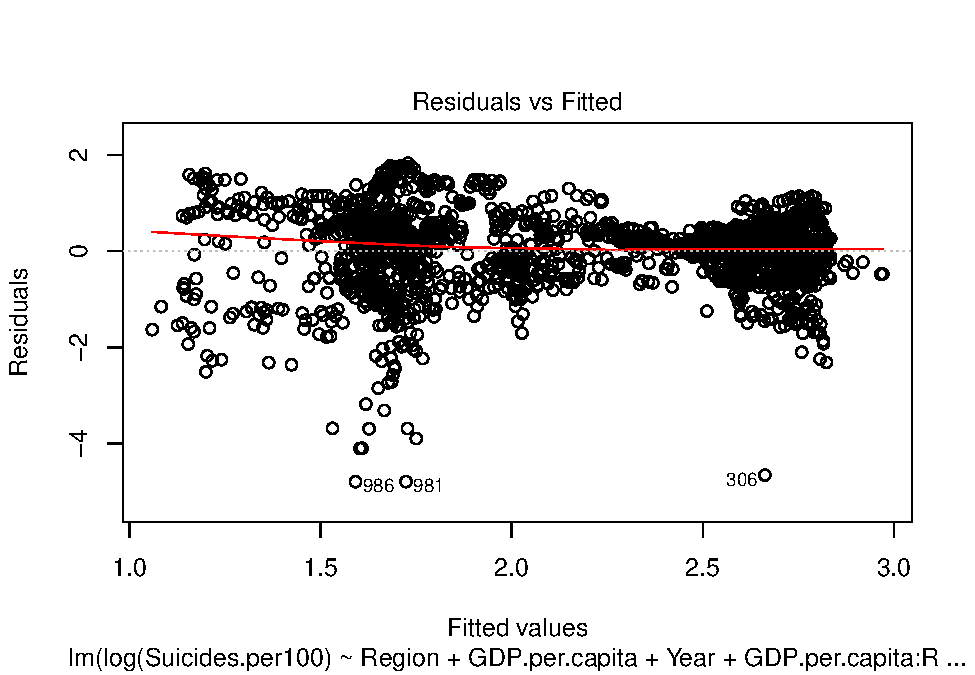
\includegraphics{LM-Homework-2_files/figure-latex/unnamed-chunk-9-1.pdf}

\begin{Shaded}
\begin{Highlighting}[]
\KeywordTok{cor}\NormalTok{(fl_crime[,}\OperatorTok{-}\DecValTok{1}\NormalTok{])}
\end{Highlighting}
\end{Shaded}

\begin{verbatim}
##                  crime education urbanization    income
## crime        1.0000000 0.4669119    0.6773678 0.4337503
## education    0.4669119 1.0000000    0.7907190 0.7926215
## urbanization 0.6773678 0.7907190    1.0000000 0.7306983
## income       0.4337503 0.7926215    0.7306983 1.0000000
\end{verbatim}

Urbanization could be this lurking variable as it has a higher
correlation between crime and education.

\hypertarget{adding-urbanization-as-a-new-variable}{%
\subsubsection{Adding urbanization as a new
variable}\label{adding-urbanization-as-a-new-variable}}

\begin{Shaded}
\begin{Highlighting}[]
\NormalTok{lm_obj_crime2 <-}\StringTok{ }\KeywordTok{lm}\NormalTok{(crime }\OperatorTok{~}\StringTok{ }\NormalTok{education }\OperatorTok{+}\StringTok{ }\NormalTok{urbanization, }\DataTypeTok{data =}\NormalTok{ fl_crime)}
\KeywordTok{summary}\NormalTok{(lm_obj_crime2)}
\end{Highlighting}
\end{Shaded}

\begin{verbatim}
## 
## Call:
## lm(formula = crime ~ education + urbanization, data = fl_crime)
## 
## Residuals:
##     Min      1Q  Median      3Q     Max 
## -34.693 -15.742  -6.226  15.812  50.678 
## 
## Coefficients:
##              Estimate Std. Error t value Pr(>|t|)    
## (Intercept)   59.1181    28.3653   2.084   0.0411 *  
## education     -0.5834     0.4725  -1.235   0.2214    
## urbanization   0.6825     0.1232   5.539 6.11e-07 ***
## ---
## Signif. codes:  0 '***' 0.001 '**' 0.01 '*' 0.05 '.' 0.1 ' ' 1
## 
## Residual standard error: 20.82 on 64 degrees of freedom
## Multiple R-squared:  0.4714, Adjusted R-squared:  0.4549 
## F-statistic: 28.54 on 2 and 64 DF,  p-value: 1.379e-09
\end{verbatim}

\begin{Shaded}
\begin{Highlighting}[]
\KeywordTok{plot}\NormalTok{(lm_obj_crime2, }\DecValTok{1}\NormalTok{)}
\end{Highlighting}
\end{Shaded}

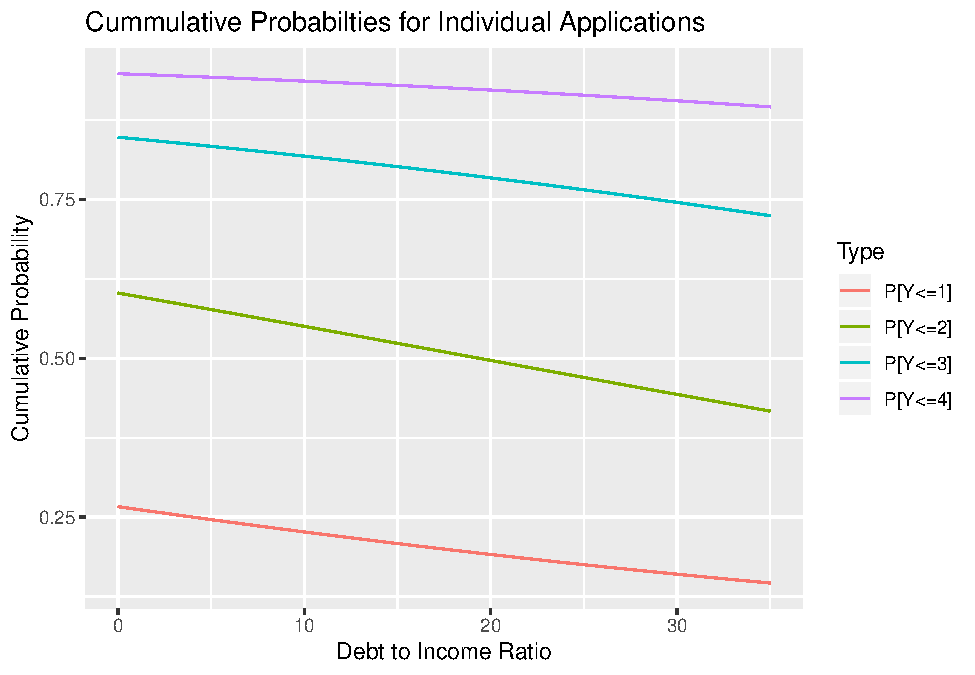
\includegraphics{LM-Homework-2_files/figure-latex/unnamed-chunk-10-1.pdf}

\begin{Shaded}
\begin{Highlighting}[]
\KeywordTok{plot}\NormalTok{(lm_obj_crime2, }\DecValTok{2}\NormalTok{)}
\end{Highlighting}
\end{Shaded}

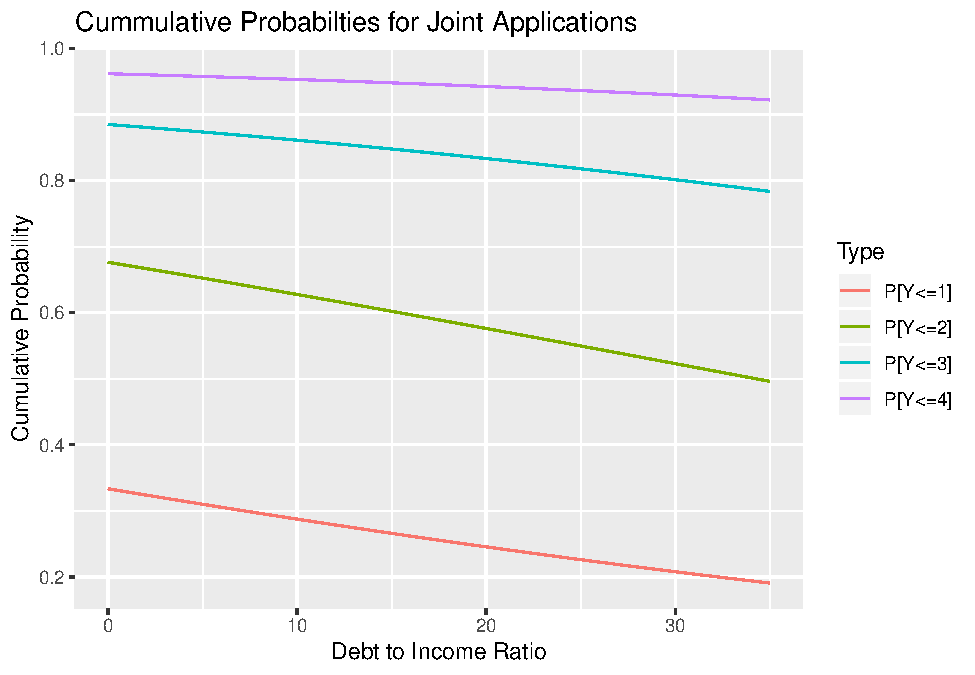
\includegraphics{LM-Homework-2_files/figure-latex/unnamed-chunk-10-2.pdf}

\hypertarget{interactive-plot}{%
\subsubsection{Interactive plot}\label{interactive-plot}}

(commented out due to markdown error)

\begin{Shaded}
\begin{Highlighting}[]
\CommentTok{#plot3d(lm_obj_crime2, size=5, col=1, data = fl_crime)}

\CommentTok{# - Add the lines showing the residuals (see "Lecture_2.R")}

\CommentTok{#plot3d(lm_obj_crime2, size=5, col=1, data = fl_crime)}

\CommentTok{#segments3d(rep(education, each=2), rep(urbanization, each=2), }
\CommentTok{#           z=matrix(t(cbind(crime,predict(lm_obj_crime2))), #nc=1), }
\CommentTok{#           add=T, }
\CommentTok{#           lwd=2, }
\CommentTok{#           col=2)}
\end{Highlighting}
\end{Shaded}

\hypertarget{prestige-data}{%
\subsection{Prestige Data}\label{prestige-data}}

\hypertarget{data-exploration}{%
\subsection{Data Exploration}\label{data-exploration}}

\begin{Shaded}
\begin{Highlighting}[]
\KeywordTok{head}\NormalTok{(Prestige)}
\end{Highlighting}
\end{Shaded}

\begin{verbatim}
##                     education income women prestige census type
## GOV.ADMINISTRATORS      13.11  12351 11.16     68.8   1113 prof
## GENERAL.MANAGERS        12.26  25879  4.02     69.1   1130 prof
## ACCOUNTANTS             12.77   9271 15.70     63.4   1171 prof
## PURCHASING.OFFICERS     11.42   8865  9.11     56.8   1175 prof
## CHEMISTS                14.62   8403 11.68     73.5   2111 prof
## PHYSICISTS              15.64  11030  5.13     77.6   2113 prof
\end{verbatim}

\begin{Shaded}
\begin{Highlighting}[]
\KeywordTok{plot}\NormalTok{(Prestige[,}\KeywordTok{c}\NormalTok{(}\OperatorTok{-}\DecValTok{5}\NormalTok{, }\DecValTok{-6}\NormalTok{)])}
\end{Highlighting}
\end{Shaded}

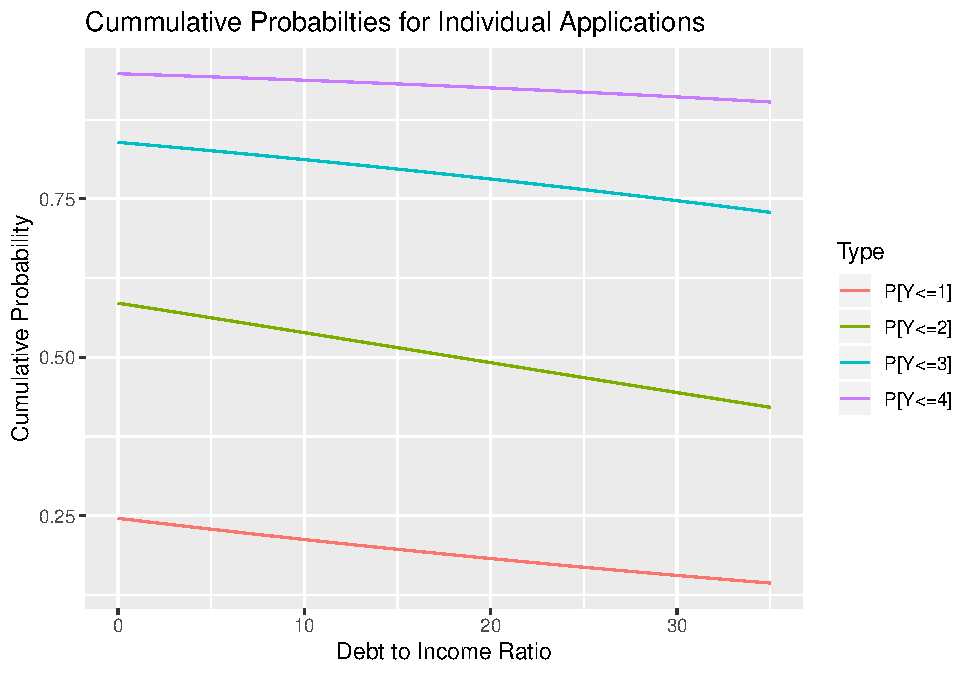
\includegraphics{LM-Homework-2_files/figure-latex/unnamed-chunk-12-1.pdf}

\begin{Shaded}
\begin{Highlighting}[]
\KeywordTok{cor}\NormalTok{(Prestige[,}\KeywordTok{c}\NormalTok{(}\OperatorTok{-}\DecValTok{5}\NormalTok{, }\DecValTok{-6}\NormalTok{)])}
\end{Highlighting}
\end{Shaded}

\begin{verbatim}
##            education     income       women   prestige
## education 1.00000000  0.5775802  0.06185286  0.8501769
## income    0.57758023  1.0000000 -0.44105927  0.7149057
## women     0.06185286 -0.4410593  1.00000000 -0.1183342
## prestige  0.85017689  0.7149057 -0.11833419  1.0000000
\end{verbatim}

Census seems to be the odd one out considering the way the values are
defined\ldots{} Otherwise, education and income have the two most
pronounced relationships with prestige. The third would be women, though
it doesn't follow very closely to the other variables.

\hypertarget{multiple-linear-regression-model}{%
\subsection{Multiple Linear Regression
Model}\label{multiple-linear-regression-model}}

\begin{Shaded}
\begin{Highlighting}[]
\NormalTok{lm_obj_prest <-}\StringTok{ }\KeywordTok{lm}\NormalTok{(prestige }\OperatorTok{~}\StringTok{ }\NormalTok{education }\OperatorTok{+}\StringTok{ }\NormalTok{income }\OperatorTok{+}\StringTok{ }\NormalTok{women, }\DataTypeTok{data =}\NormalTok{ Prestige)}
\KeywordTok{summary}\NormalTok{(lm_obj_prest)}
\end{Highlighting}
\end{Shaded}

\begin{verbatim}
## 
## Call:
## lm(formula = prestige ~ education + income + women, data = Prestige)
## 
## Residuals:
##      Min       1Q   Median       3Q      Max 
## -19.8246  -5.3332  -0.1364   5.1587  17.5045 
## 
## Coefficients:
##               Estimate Std. Error t value Pr(>|t|)    
## (Intercept) -6.7943342  3.2390886  -2.098   0.0385 *  
## education    4.1866373  0.3887013  10.771  < 2e-16 ***
## income       0.0013136  0.0002778   4.729 7.58e-06 ***
## women       -0.0089052  0.0304071  -0.293   0.7702    
## ---
## Signif. codes:  0 '***' 0.001 '**' 0.01 '*' 0.05 '.' 0.1 ' ' 1
## 
## Residual standard error: 7.846 on 98 degrees of freedom
## Multiple R-squared:  0.7982, Adjusted R-squared:  0.792 
## F-statistic: 129.2 on 3 and 98 DF,  p-value: < 2.2e-16
\end{verbatim}

\(\hat{prestige_i} = -6.794 + 4.187(education_i) + 0.00131(income_i) - 0.0089(women_i)\)

Interpretations:

intercept - doesn't make much sense to interpret

education - on average and holding all other variables constant, for
every one year increase in education, we predict the prestige score to
increase by 4.187 points.

income - on average and holding all other variables constant, for every
one dollar increase in income, we predict the prestige score to increase
by 0.0013 points

women - on average and holding all other variables constant, for every
one percentage point increase in the number of incumbents who are women,
we predict the prestige score to decrease by 0.0089 points

\(R^2\) - 79.82\% of the variance in prestige is explained by our model

RSE - on average, our predictions are off by 7.846 Ineo-Porter prestige
score points

\hypertarget{standardize-slopes}{%
\subsection{Standardize slopes}\label{standardize-slopes}}

\begin{Shaded}
\begin{Highlighting}[]
\NormalTok{scaled_Prestige <-}\StringTok{ }\KeywordTok{data.frame}\NormalTok{(}\KeywordTok{scale}\NormalTok{(Prestige[,}\KeywordTok{c}\NormalTok{(}\OperatorTok{-}\DecValTok{5}\NormalTok{,}\OperatorTok{-}\DecValTok{6}\NormalTok{)]))}
\NormalTok{lm_obj_prest2 <-}\StringTok{ }\KeywordTok{lm}\NormalTok{(prestige }\OperatorTok{~}\StringTok{ }\NormalTok{education }\OperatorTok{+}\StringTok{ }\NormalTok{income }\OperatorTok{+}\StringTok{ }\NormalTok{women, }\DataTypeTok{data =}\NormalTok{ scaled_Prestige)}
\KeywordTok{coef}\NormalTok{(lm_obj_prest2)}
\end{Highlighting}
\end{Shaded}

\begin{verbatim}
##   (Intercept)     education        income         women 
## -1.396196e-17  6.639551e-01  3.241757e-01 -1.642104e-02
\end{verbatim}

Education has the greatest practical effect on prestige, followed by
income.

\end{document}
